\documentclass[conference]{IEEEtran}

% Paquetes
\usepackage[utf8]{inputenc}
\usepackage[spanish]{babel}
\usepackage{amsmath,amssymb}
\usepackage{graphicx}
\usepackage{booktabs}       
\usepackage{hyperref}
\usepackage{url}
\usepackage{float}          
\usepackage{multirow}       
\usepackage{array}

% Info inicial
\title{Sistema de Recomendación de Vehículos Usados Basado en 
Machine Learning e Integrado en un Agente Inteligente}

\author{
    \IEEEauthorblockN{Andrés Bonilla Solano}
    \IEEEauthorblockA{
        Escuela de Ingeniería en Computación\\
        Instituto Tecnológico de Costa Rica\\
        Cartago, Costa Rica\\
        andbonilla@estudiantec.cr
    }
    \and
    \IEEEauthorblockN{Mary Paz Álvarez Navarrete}
    \IEEEauthorblockA{
        Escuela de Ingeniería en Computación\\
        Instituto Tecnológico de Costa Rica\\
        Cartago, Costa Rica\\
        mar01alvarez@estudiantec.cr
    }
}

% Inicio de documento
\begin{document}
\maketitle

% ABSTRACT
\begin{abstract}
La compra de vehículos usados representa una decisión financiera significativa para los consumidores, especialmente en contextos donde el acceso a vehículos nuevos está limitado por su costo. Sin embargo, el mercado carece de herramientas accesibles que permitan evaluar objetivamente la relación calidad-precio de un vehículo. Este trabajo presenta un sistema de recomendación basado en LightGBM, entrenado sobre 364{,}546 registros reales de Craigslist, que estima el valor de mercado de vehículos usados a partir de sus características. El modelo final obtuvo un MAE de \$3{,}999 y un R² de 0.762 sobre el conjunto de prueba, superando el baseline de regresión lineal en un 27.4\%. El modelo fue integrado en un agente inteligente construido con LangGraph, con arquitectura Planner-Executor-Verifier, que recibe consultas en lenguaje natural mediante el modelo Qwen3 ejecutado localmente, invoca el modelo como herramienta y retorna recomendaciones justificadas mediante explicaciones SHAP. La validación del agente sobre 21 turnos de conversación estructurada alcanzó una tasa de éxito global del 81\%, con 100\% en las tareas de estimación de precio y explicación de predicciones.
\end{abstract}

% KEYWORDS
\begin{IEEEkeywords}
Machine Learning, LightGBM, Sistema de Recomendación, SHAP, Agente Inteligente, Vehículos Usados, Gradient Boosting, Planner, Executor, Verifier, LangGraph
\end{IEEEkeywords}

% INTRODUCCIÓN
\section{Introducción}

La adquisición de vehículos usados es parte de una de las decisiones financieras más significativas para los consumidores, especialmente en situaciones donde el acceso a vehículos nuevos es limitado por su costo. En mercados como el estadounidense, plataformas de clasificados en línea como Craigslist concentran numerosos anuncios de venta con distintas características, lo que hace difícil que un comprador pueda evaluar desde un punto de vista objetivo si un vehículo representa una oferta razonable dentro de su presupuesto.

El precio de un vehículo usado no puede calcularse de una manera sencilla, debido a que depende de la interacción no lineal de múltiples  factores: el año de fabricación, el kilometraje acumulado, la marca, el tipo de carrocería, el estado mecánico y las condiciones del mercado regional, entre otros. Esto hace que los enfoques basados en heurísticas o modelos lineales no sean suficientes para capturar la variabilidad real del mercado, ya que depende de varios factores.

Ante esta problemática, se propone un sistema de recomendación de vehículos usados basado en técnicas de aprendizaje automático, diseñado para asistir a los compradores en la identificación de vehículos con una relación calidad-precio favorable. El sistema fue desarrollado a partir de un conjunto de datos de 426,880 registros reales provenientes de Craigslist \cite{sulianta2024}, el cual fue sometido a un proceso exhaustivo de limpieza y preprocesamiento que redujo el conjunto de datos a 364,546 registros utilizables. Sobre este conjunto se evaluaron seis modelos de aprendizaje automático, incluyendo Regresión Lineal, Ridge Regression, Decision Tree, Random Forest, XGBoost y LightGBM, mediante un protocolo de validación temporal estricto. Como resultado, LightGBM \cite{ke2017} fue seleccionado como modelo principal al demostrar el mejor equilibrio entre precisión predictiva y capacidad de generalización. Posteriormente, el modelo fue optimizado mediante búsqueda aleatoria de hiperparámetros y evaluado sobre un conjunto de prueba independiente, obteniendo un error absoluto medio de \$4,000 y un coeficiente de determinación (R²) de 0.762. Estos resultados representan una mejora del 27.4\% con respecto al modelo de referencia.

Como componente transversal del sistema, el modelo fue integrado en un agente inteligente construido con LangGraph siguiendo una arquitectura Planner-Executor-Verifier. El \textit{Planner} utiliza el modelo de lenguaje Qwen3 ejecutado localmente mediante Ollama para interpretar consultas en lenguaje natural y extraer parámetros estructurados. El \textit{Executor} invoca el modelo predictivo como herramienta y el \textit{Verifier} valida la coherencia del resultado antes de retornar una respuesta justificada con explicaciones SHAP \cite{lundberg2017}. Esta integración permite que el sistema no solo prediga precios, sino que explique al usuario los factores que determinan el valor estimado de cada vehículo.

Las contribuciones principales de este trabajo son las siguientes:

\begin{itemize}
\item El desarrollo de un pipeline reproducible para la predicción de precios de vehículos usados, incorporando estrategias para prevenir \textit{data leakage} por medio de la partición temporal de los datos.

\item La evaluación comparativa de varios modelos de aprendizaje automático por medio de un protocolo de validación temporal, considerando tanto el desempeño predictivo como su capacidad de generalización.

\item La aplicación de técnicas de explicabilidad basadas en SHAP para identificar los factores más influyentes en la estimación de precios.

\item La integración del modelo predictivo en un agente inteligente con arquitectura Planner-Executor-Verifier construido con LangGraph, que permite consultas en lenguaje natural, recomendaciones justificadas y explicaciones SHAP por predicción individual.
\end{itemize}

Dentro del articulo se encuentran las siguientes secciones: la Sección~\ref{sec:related} presenta los trabajos relacionados; la Sección~\ref{sec:metodologia} describe la metodología empleada; la Sección~\ref{sec:resultados} reporta los experimentos y resultados obtenidos; la Sección~\ref{sec:discusion} discute los hallazgos principales y las limitaciones del sistema; y la Sección~\ref{sec:conclusiones} presenta las conclusiones y el trabajo futuro.

% TRABAJOS RELACIONADOS
\section{Trabajos Relacionados}
\label{sec:related}

% Predicción de precios de vehículos usados
La predicción de precios de vehículos usados mediante aprendizaje automático ha sido abordada desde múltiples enfoques. Cui et al.~\cite{cui2022} propusieron un marco iterativo que combina XGBoost y LightGBM para la predicción de precios bajo grandes volúmenes de características, fusionando las predicciones de una red residual profunda con las features originales como entrada al marco iterativo. Sus experimentos demostraron que esta combinación supera al Random Forest y a las redes residuales individuales en precisión. A diferencia de este enfoque, este trabajo evalúa cada modelo de forma independiente por medio de un protocolo de validación temporal estricto, priorizando la capacidad de generalización sobre datos futuros mediante el análisis del Gap R² como métrica de overfitting.

De igual manera, trabajos previos han comparado múltiples modelos de aprendizaje automático para este problema, incluyendo regresión lineal, K-Nearest Neighbors, Random Forest y XGBoost sobre datasets de vehículos usados de diversas regiones \cite{ijert2022}. Estos estudios coinciden en que los modelos basados en árboles de decisión  superan consistentemente a los modelos lineales, confirmando que es necesario generar relaciones no lineales entre las variables del mercado automotriz. Sin embargo, la mayoría de estos trabajos no implementan partición temporal de los datos ni analizan el riesgo de   data leakage, limitaciones que el presente trabajo aborda explícitamente.

% Algoritmos de boosting
El algoritmo XGBoost, propuesto por Chen y Guestrin~\cite{chen2016}, introdujo un sistema escalable de gradient boosting basado en árboles  con optimizaciones de caché, compresión de datos y soporte para datos dispersos. Su uso en competencias de aprendizaje automático lo convirtió en el punto de referencia para datos tabulares. Después, Ke et al.~\cite{ke2017} propusieron LightGBM, que supero a XGBoost en eficiencia mediante dos innovaciones algorítmicas: \textit{Gradient-based One-Side Sampling} (GOSS), que reduce el tamaño del conjunto de entrenamiento dando prioridad a instancias con gradientes grandes, y \textit{Exclusive Feature Bundling} (EFB), que reduce el número de features agrupando variables mutuamente excluyentes. Los experimentos de los autores demuestran que LightGBM acelera el entrenamiento hasta 20 veces respecto a GBDT convencional manteniendo una precisión comparable. En el presente trabajo se confirma esta ventaja de velocidad: LightGBM completó la validación cruzada en 11 segundos frente a los 76 segundos de Random Forest sobre un dataset de 255{,}182 registros.

% Explicabilidad con SHAP 
La explicabilidad de los modelos de aprendizaje automático ha cobrado relevancia creciente en aplicaciones de alto impacto donde las decisiones deben ser auditables y comprensibles para los usuarios finales. Lundberg y Lee~\cite{lundberg2017} propusieron SHAP (SHapley Additive exPlanations), un marco unificado para la interpretación de predicciones individuales basado en valores de Shapley de la teoría de juegos. SHAP asigna a cada feature un valor de importancia para una predicción específica, con la propiedad de que la suma de todos los valores SHAP reproduce exactamente la predicción del modelo. A diferencia de métodos anteriores como LIME, SHAP presenta consistencia teórica garantizada y permite tanto explicaciones locales (por predicción) como globales (sobre todo el dataset). En el presente trabajo se aplica \texttt{TreeExplainer}, la variante optimizada de SHAP para modelos basados en árboles, sobre una muestra de 2{,}000 registros del conjunto de prueba. Los resultados revelan que el año y el kilometraje dominan las predicciones de precio, confirmando las correlaciones identificadas en el análisis exploratorio y validando la coherencia del modelo con el conocimiento del dominio.

% Integración del agente
La integración de modelos predictivos en agentes inteligentes representa una tendencia emergente en la literatura. Trabajos recientes han demostrado que los LLMs pueden actuar como orquestadores de herramientas externas mediante \textit{tool calling}, descomponiendo tareas complejas en subtareas manejables y seleccionando las herramientas apropiadas para cada una \cite{schick2023, masterman2024}. En particular, la arquitectura Planner-Executor ha demostrado robustez en escenarios de uso real \cite{dong2025}, mientras que la incorporación de un nodo Verifier agrega una capa de validación que mejora la confiabilidad del sistema ante entradas ambiguas o casos límite \cite{chu2024}. A diferencia de los sistemas de recomendación tradicionales basados en filtrado colaborativo \cite{aggarwal2016}, el enfoque propuesto emplea el modelo de predicción de precios como herramienta del agente, permitiendo recomendaciones justificadas con explicaciones SHAP que detallan los factores determinantes del precio estimado para cada vehículo.

% METODOLOGÍA
\section{Metodología}
\label{sec:metodologia}

%----------------------------------------------------
\subsection{Dataset y Preprocesamiento}
\label{subsec:dataset}
El dataset utilizado corresponde a anuncios de vehículos usados publicados en la plataforma de Craigslist, recopilado por Austin Reese y disponible en Kaggle. Originalmente contiene 426 880 registros y 26 variables que describen las características del vehículo y del anuncio. Luego de realizar un análisis, se determinó que existían columnas sin valor predictivo o con riesgo de \textit{data leakage} por lo que no se tomaron en cuenta. Las nueve columnas eliminadas son: \texttt{id}, \texttt{url}, \texttt{region\_url}, \texttt{image\_url}, \texttt{VIN}, \texttt{lat}, \texttt{long}, \texttt{county} y \texttt{description}. La razón para borrar la columna que contiene la descripción es que frecuentemente contiene el precio del vehículo de forma explícita en el texto libre del vendedor. Se aplicaron filtros de valores atípicos basados en rangos lógicos del mercado: precio entre \$500 y \$100 000, odómetro entre 100 y 500 000 millas, y año de fabricación entre 1990 y 2022. La columna \texttt{size} fue eliminada por presentar un 71.77\% de valores nulos, umbral a partir del cual la imputación introduce ruido artificial. Para las columnas \texttt{cylinders}, \texttt{condition} y \texttt{drive}, con porcentajes de nulos entre 30\% y 42\%, se aplicó imputación por moda agrupada según el fabricante y el tipo de vehículo, dado que vehículos de características similares tienden a compartir estos atributos. Tras aplicar todos los filtros, el dataset quedó conformado por 364 546 registros listos para ser usados en las siguientes partes del proyecto.


%----------------------------------------------------
\subsection{Pipeline de Transformación}
\label{subsec:pipeline}
Las variables de entrada se organizaron en tres grupos según su naturaleza y el tratamiento que requieren. Las variables numéricas \texttt{year} y \texttt{odometer} se normalizaron con \texttt{StandardScaler} para garantizar que las features sigan una distribución normal estándar. También, hay variables categóricas con orden semántico inherente, como es el caso de \texttt{condition} y \texttt{cylinders}, se codificaron con \texttt{OrdinalEncoder} respetando sus jerarquías naturales. Para la condición, las categorías van de vehículos declarados como pérdida total hasta otros que pueden ser catalogados como nuevos, y de 3 a 12 cilindros en el caso de cilindrada. El resto de variables categóricas no tienen un orden natural (\texttt{manufacturer}, \texttt{fuel}, \texttt{transmission}, \texttt{drive}, \texttt{type}, \texttt{title\_status}) por lo que se codificaron con \texttt{OneHotEncoder} y con \texttt{drop=`first'} para evitar multicolinealidad en los modelos lineales. Todo el preprocesamiento se encapsuló en un \texttt{ColumnTransformer} integrado dentro de un \texttt{Pipeline} de scikit-learn junto al modelo de predicción. Con el fin de prevenir el \textit{data leakage} se tomó esta decisión de usar un pipeline ya que los parámetros de escalado, imputación y codificación se aprenden exclusivamente con los datos de entrenamiento y se aplican posteriormente al conjunto de validación y prueba. Finalmente, el resultado tras la expansión por el uso del \texttt{OneHotEncoder} es un espacio de 67 de features.

%----------------------------------------------------
\subsection{Partición Temporal}
\label{subsec:particion}
Para el presente proyecto se adoptó una estrategia de partición temporal basada en la columna \texttt{posting\_date} ya que para este caso es mejor que una partición aleatoria. Esto se debe a que si se usa una partición aleatoria se permitiría que el modelo entrene con anuncios publicados después de los que se usan para evaluación, lo que llevaría a simular un conocimiento del futuro que no existe en producción. Asimismo, el dataset se ordenó cronológicamente y se dividió en tres conjuntos contiguos y no solapados: 70\% de los registros más antiguos para entrenamiento (255 182 registros, hasta el 30 de abril de 2021), 15\% intermedios para validación durante el ajuste de hiperparámetros (54 681 registros, del 30 de abril al 3 de mayo de 2021), y 15\% más recientes para la prueba final (54 683 registros, del 3 al 5 de mayo de 2021). Es importante mencionar que el conjunto de prueba se utilizó únicamente para la evaluación final del modelo seleccionado, garantizando que ninguna decisión de diseño o ajuste de hiperparámetros fue influenciada por su contenido. 

%----------------------------------------------------
\subsection{Modelos y Protocolo de Evaluación}
\label{subsec:modelos}

Se evaluaron seis modelos de aprendizaje automático bajo un protocolo unificado de validación cruzada temporal. Para garantizar que las diferencias en rendimiento sean exclusivamente al modelo y no al preprocesamiento, todos los modelos reciben el mismo \texttt{ColumnTransformer} definido en la subsección anterior como primera etapa de un \texttt{Pipeline} de scikit-learn.

El protocolo de evaluación consiste en un esquema de validación \texttt{TimeSeriesSplit} con $k=5$ folds sobre el conjunto de entrenamiento, respetando el orden cronológico en cada partición. Se calculan tres métricas por modelo: MAE, RMSE y R². Además, se reporta el Gap en R², definido como la diferencia entre el R² sobre el conjunto de entrenamiento y el R² sobre el conjunto de validación:

\begin{equation}
    \text{Gap-}R^2 = R^2_{\text{train}} - R^2_{\text{val}}
    \label{eq:gap}
\end{equation}

Un Gap R² elevado indica que el modelo memoriza los datos de entrenamiento en lugar de aprender patrones generalizables, conocido como \textit{overfitting}. Se establece como umbral de alerta un Gap R² superior a 0.10.

Los seis modelos evaluados y sus configuraciones iniciales son los siguientes:

\textbf{Regresión Lineal (Baseline 1):} Modelo de referencia mínimo que asume relaciones lineales entre las variables y el precio. Sirve para cuantificar cuánto se puede explicar sin capturar no-linealidades.

\textbf{Ridge Regression (Baseline 2):} Extensión regularizada de la regresión lineal con penalización L2 ($\alpha{=}1.0$). Mitiga los coeficientes extremos generados por categorías poco frecuentes como marcas de lujo con pocos registros en el dataset.

\textbf{Decision Tree:} Árbol de decisión con profundidad máxima de cinco niveles y un mínimo de 50 muestras por hoja (\texttt{max\_depth=5}, \texttt{min\_samples\_leaf=50}). Se incluye por su valor interpretativo, ya que permite visualizar directamente la lógica de decisión del modelo en los primeros tres niveles.

\textbf{Random Forest:} Ensemble de 100 árboles de decisión entrenados sobre muestras aleatorias del dataset mediante bagging (\texttt{n\_estimators=100}, \texttt{min\_samples\_leaf=5}). Captura relaciones no lineales sin transformaciones manuales, por ejemplo la depreciación exponencial observada en el EDA entre año de fabricación y precio.

\textbf{XGBoost:} Algoritmo de gradient boosting que construye árboles de forma secuencial por niveles (\textit{depth-wise}) \cite{chen2016}. Se configura con 300 árboles, tasa de aprendizaje de 0.05, profundidad máxima de 6 y submuestreo de 80\% tanto de filas (\texttt{subsample}) como de features (\texttt{colsample\_bytree}) por árbol.

\textbf{LightGBM:} Algoritmo de gradient boosting que divide los árboles por hojas (\textit{leaf-wise}) en lugar de por niveles, logrando mayor velocidad y precisión en datasets grandes \cite{ke2017}. Se configura con 300 árboles, tasa de aprendizaje de 0.05 y 63 hojas por árbol (\texttt{num\_leaves=63}).

Los resultados de la comparación se presentan en la Tabla~\ref{tab:modelos}. Random Forest obtiene el menor MAE (\$3{,}798), pero con un Gap R² de 0.124 que indica overfitting moderado. LightGBM alcanza el mayor R² (0.798) con un Gap R² de 0.058, superando a Random Forest en capacidad de generalización con una diferencia en MAE de solo \$189 (4.7\%). La velocidad de entrenamiento de LightGBM (22s frente a 179s de Random Forest) hace que el proceso de optimización de hiperparámetros sea 8 veces más rápido. Por estas razones, LightGBM es seleccionado como modelo principal para la siguiente etapa.

%----------------------------------------------------
\subsection{Optimización de Hiperparámetros}
\label{subsec:hypertuning}

La optimización de hiperparámetros se realizó mediante \texttt{RandomizedSearchCV} sobre LightGBM, utilizando el mismo protocolo de \texttt{TimeSeriesSplit} $k{=}5$ empleado en la evaluación de candidatos. Se optó por búsqueda aleatoria en lugar de búsqueda exhaustiva (\texttt{GridSearchCV}) dado que el espacio de seis hiperparámetros con los rangos definidos implica un número de combinaciones que haría inviable la evaluación completa con el tamaño del dataset. Con 50 iteraciones aleatorias y 5 folds por iteración se realizaron 250 entrenamientos en total, con una duración de aproximadamente 24 minutos por ronda de búsqueda.

El espacio de búsqueda definido fue el siguiente:

\begin{itemize}
    \item \texttt{n\_estimators}: entero uniforme en $[200, 800]$
    \item \texttt{learning\_rate}: continuo uniforme en $[0.01, 0.20]$
    \item \texttt{num\_leaves}: entero uniforme en $[20, 150]$
    \item \texttt{min\_child\_samples}: entero uniforme en $[20, 200]$
    \item \texttt{subsample}: continuo uniforme en $[0.60, 1.00]$
    \item \texttt{colsample\_bytree}: continuo uniforme en $[0.60, 1.00]$
\end{itemize}

La primera búsqueda (\textit{Tuning v1}) encontró parámetros agresivos: \texttt{learning\_rate=0.181}, \texttt{num\_leaves=118} y \texttt{min\_child\_samples=28}. Esta combinación redujo el MAE de \$3{,}987 a \$3{,}588, pero aumentó el Gap R² de 0.058 a 0.102, indicando mayor overfitting que el modelo sin afinar. El \texttt{learning\_rate} elevado genera correcciones grandes en cada ronda de boosting, lo que favorece la memorización de patrones específicos del conjunto de entrenamiento.

Debido a este resultado, se realizó una segunda búsqueda (\textit{Tuning v2}) con rangos más conservadores: \texttt{learning\_rate} limitado a $[0.01, 0.08]$, \texttt{num\_leaves} a $[20, 80]$ y \texttt{min\_child\_samples} elevado a $[50, 300]$. Para compensar el menor ritmo de aprendizaje, el rango de \texttt{n\_estimators} se amplió a $[400, 900]$. Los mejores parámetros encontrados fueron: \texttt{learning\_rate=0.073}, \texttt{num\_leaves=67}, \texttt{min\_child\_samples=63}, \texttt{n\_estimators=750}, \texttt{subsample=0.714} y \texttt{colsample\_bytree=0.929}.

El modelo resultante (\textit{Tuning v2}) obtuvo un MAE de \$3{,}660 sobre el conjunto de validación, con un Gap R² de 0.074, reducción del 27.6\% respecto al gap de \textit{Tuning v1}. Los resultados comparativos de las tres versiones de LightGBM se presentan en la Tabla~\ref{tab:hypertuning}. Se selecciona \textit{Tuning v2} como modelo final por representar el mejor balance entre precisión (\$327 de mejora en MAE respecto al modelo sin afinar) y capacidad de generalización (Gap R² de 0.074 frente a 0.102 de \textit{Tuning v1}).

%----------------------------------------------------
\subsection{Explicabilidad con SHAP}
\label{subsec:shap}

Para garantizar la interpretabilidad del modelo final se aplicó SHAP (\textit{SHapley Additive exPlanations}) \cite{lundberg2017}, un marco unificado de explicabilidad basado en la teoría de juegos de Shapley. SHAP asigna a cada feature un valor de importancia para cada predicción individual, con la propiedad de que la suma de todos los valores SHAP reproduce exactamente la predicción del modelo, lo que garantiza consistencia local y global.

Se utilizó \texttt{TreeExplainer}, la variante optimizada de SHAP para modelos basados en árboles, aplicada sobre el modelo final \textit{LightGBM Tuning v2}. Dado que SHAP requiere datos en formato numérico, se transformó previamente \texttt{X\_test} mediante el \texttt{ColumnTransformer} del pipeline. El análisis se realizó sobre una muestra aleatoria de 2{,}000 registros del conjunto de prueba (semilla SEED=42) para mantener la viabilidad computacional.

Se generaron tres visualizaciones complementarias. El \textit{summary plot} muestra la distribución de los valores SHAP para las 15 features más influyentes sobre toda la muestra, donde el color codifica el valor real de la variable (rojo para valores altos, azul para valores bajos) y el eje horizontal representa el impacto en dólares sobre el precio predicho. El \textit{bar plot} presenta el ranking de importancia como el promedio del valor absoluto de SHAP por feature, permitiendo una lectura directa de la magnitud de influencia de cada variable. Finalmente, el \textit{waterfall plot} desglosa la predicción individual del vehículo con precio más cercano a la mediana del mercado (\$14{,}444), mostrando la contribución positiva o negativa de cada feature desde el precio base de \$19{,}809 hasta el precio predicho de \$14{,}287, con un error de solo \$157.

Los resultados del análisis SHAP y su interpretación se presentan en la Sección~\ref{sec:discusion}.

%----------------------------------------------------
\subsection{Integración en Agente Inteligente}
El modelo desarrollado en la segunda etapa del proyecto fue integrado en un sistema multiagente construido con LangGraph, un framework de orquestación de agentes basado en grafos de estado. La arquitectura implementada sigue un patrón secuencial de tres nodos especializados: \textit{Planner}, \textit{Executor} y \textit{Verifier}, coordinados a través de un estado compartido tipado (\texttt{EstadoAgente}) que elimina la necesidad de variables globales. Asimismo, la memoria persistente entre turnos se implementó mediante \texttt{MemorySaver} disponible en LangGraph. Esto lo que permite es que el agente pueda mantener el contexto de conversaciones de múltiples intercambios dentro de una misma sesión.

Primero, el \textit{Planner} utiliza el modelo de lenguaje Qwen3 ejecutado localmente mediante Ollama, lo que elimina la dependencia de APIs externas y garantiza la reproducibilidad del sistema. En esta parte, se recibe la consulta del usuario en lenguaje natural junto con el historial reciente de la conversación, y se produce un plan en formato JSON basado en los datos extraídos que especifica la tarea a ejecutar, los parámetros y metadatos como el modelo exacto del vehículo (característica que no es usada por su alta cardinalidad). Al incluir el modelo exacto como metadato se evita que el \textit{Executor} intente usarla como feature. Se definieron tres tareas posibles: \texttt{estimar\_precio}, \texttt{buscar\_vehiculos} y \texttt{explicar\_prediccion}.

El \textit{Executor} actúa como puente entre el grafo y las herramientas de predicción. Recibe la tarea y los parámetros del estado compartido y los mapea a tres funciones especializadas: \texttt{buscar\_vehiculos}, que filtra el dataset según los criterios del usuario y ordena los resultados por una puntuación de calidad-precio; \texttt{estimar\_precio}, que invoca el pipeline completo de LightGBM Tuning v2 para predecir el valor de mercado; y \texttt{explicar\_prediccion}, que aplica \texttt{TreeExplainer} de SHAP sobre la predicción para descomponer los factores que determinaron el precio estimado. Adicionalmente, se implementó un filtro de coherencia que evalúa cada registro del dataset comparando su precio real contra la predicción del modelo, excluyendo anuncios con errores relativos superiores al 500\% que corresponden a precios simbólicos o errores de publicación.

El \textit{Verifier} opera en dos niveles. En el nivel de errores críticos, detecta fallos del \textit{Executor} y ausencia de  resultados, activando un mecanismo de reintento automático con hasta dos intentos por turno, en los que relaja progresivamente los filtros de búsqueda en el siguiente orden: condición mínima, combustible, transmisión, fabricante, año mínimo y precio máximo. En el nivel de advertencias, corrige automáticamente errores tipográficos en valores categóricos (como \texttt{excelent} a \texttt{excellent}), valida que los valores extraídos pertenezcan a los conjuntos permitidos por el dataset, y notifica al usuario sobre disponibilidad limitada o uso de valores por defecto. Finalmente, el \textit{Verifier} formatea la respuesta final con la información estructurada del resultado y las advertencias aplicables antes de retornarla al usuario \cite{rosario2025}.


% EXPERIMENTOS Y RESULTADOS
\section{Experimentos y Resultados}
\label{sec:resultados}

\subsection{Comparación de Modelos Candidatos}
\label{subsec:comparacion}

Se evaluaron seis modelos mediante validación cruzada temporal (\texttt{TimeSeriesSplit} $k{=}5$) sobre el conjunto de entrenamiento de 255{,}182 registros. La Tabla~\ref{tab:modelos} presenta los resultados consolidados ordenados por MAE ascendente.

\begin{table}[H]
    \centering
    \caption{Comparación de modelos - Validation Set (CV $k{=}5$)}
    \label{tab:modelos}
    \begin{tabular}{lrrrr}
        \toprule
        \textbf{Modelo} & \textbf{MAE (\$)} & \textbf{R²} & \textbf{Gap R²} & \textbf{t(s)} \\
        \midrule
        Random Forest        & 3{,}798 & 0.797 & 0.124 & 179 \\
        LightGBM             & 3{,}987 & 0.798 & 0.058 & 22  \\
        XGBoost              & 4{,}157 & 0.786 & 0.044 & 30  \\
        Reg. Lineal (B1)     & 5{,}510 & 0.655 & —     & —   \\
        Ridge (B2)           & 5{,}633 & 0.670 & 0.017 & 6   \\
        Decision Tree        & 5{,}866 & 0.637 & 0.019 & 6   \\
        \bottomrule
    \end{tabular}
\end{table}

Los modelos basados en árboles de decisión no lineales (Random Forest, LightGBM y XGBoost) superan consistentemente a los modelos lineales (Regresión Lineal y Ridge) en todas las métricas, con reducciones en MAE de entre \$1{,}551 y \$2{,}068 respecto al mejor baseline. Este resultado confirma que las relaciones entre las variables del mercado de vehículos usados no son capturables mediante transformaciones lineales, tal como sugería la tendencia exponencial observada en el diagrama de dispersión precio-año del EDA.

Random Forest obtiene el menor MAE (\$3{,}798) pero presenta el mayor Gap R² (0.124), lo que indica overfitting moderado, su R² en entrenamiento es de 0.921 frente a 0.797 en validación. LightGBM alcanza el R² más alto (0.798) con un Gap R² de 0.058, lo que representa la mitad del overfitting de Random Forest, con una diferencia de MAE de solo \$189 (4.7\%). XGBoost exhibe el menor Gap R² de todos los modelos no lineales (0.044), pero su MAE es \$370 superior al de LightGBM y su R² es 0.012 inferior. Por las razones expuestas en la Subsección~\ref{subsec:hypertuning}, LightGBM es seleccionado como modelo principal para la optimización de hiperparámetros.

\begin{figure}[H]
    \centering
    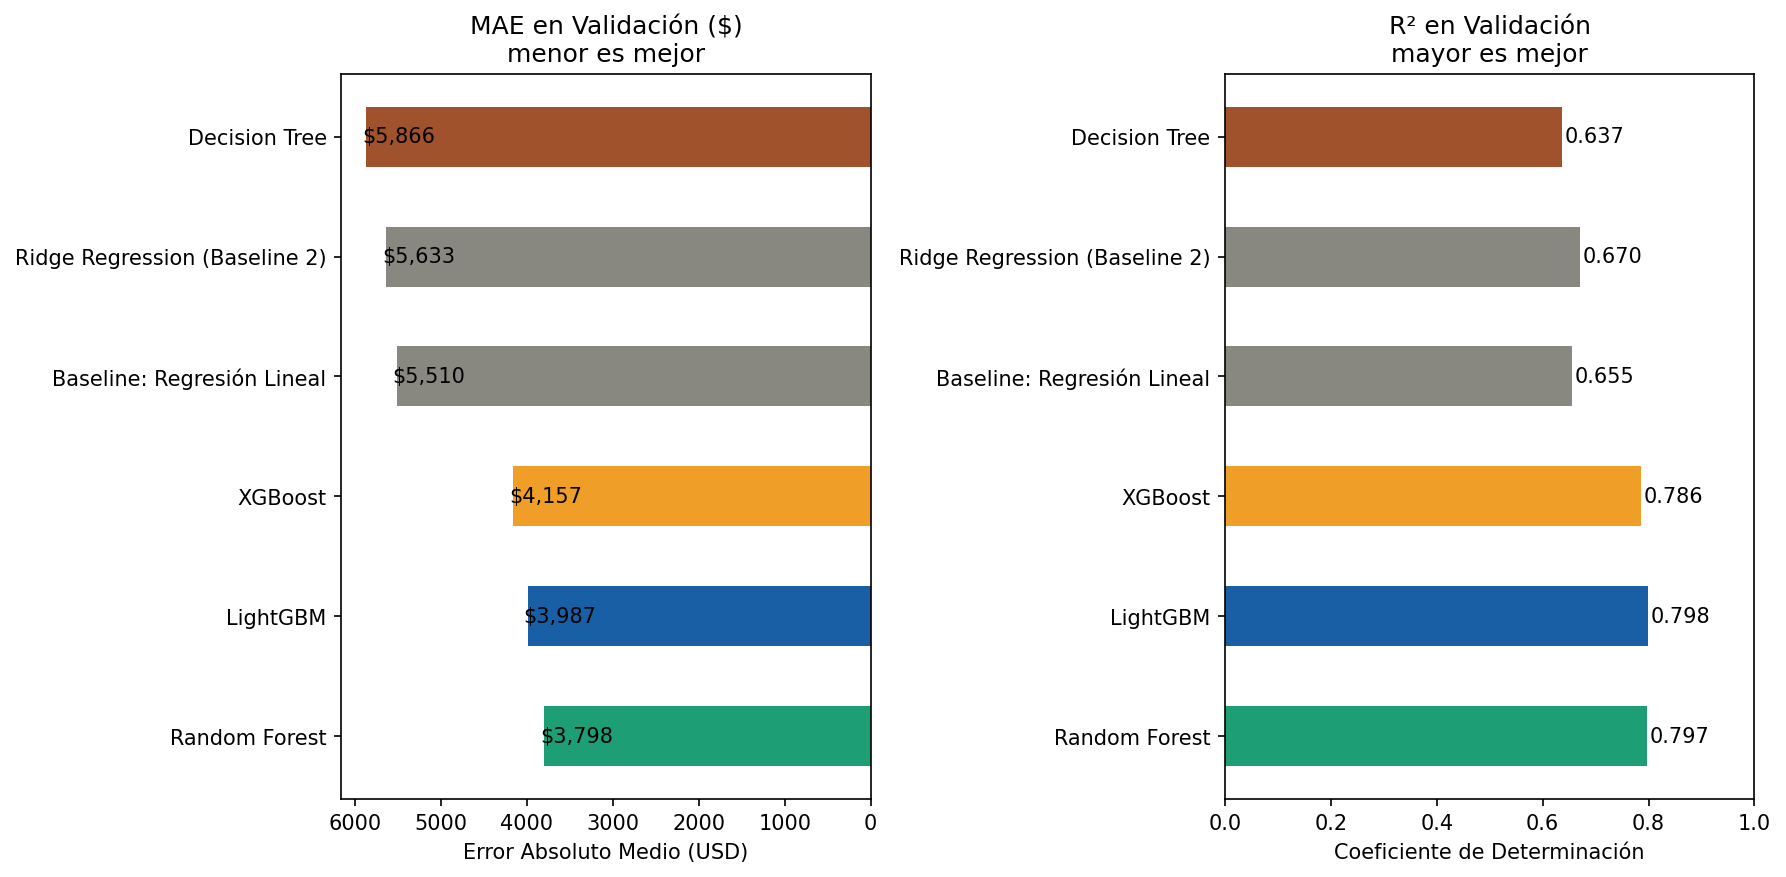
\includegraphics[width=\columnwidth]{../SegundaEtapa/comparacion_modelos.png}
    \caption{Comparación de MAE y R² en validación para los seis modelos evaluados.}
    \label{fig:comparacion}
\end{figure}


%----------------------------------------------------
\subsection{Optimización de Hiperparámetros}
\label{subsec:res_hypertuning}

La Tabla~\ref{tab:hypertuning} presenta los resultados de las dos rondas de búsqueda aleatoria sobre el conjunto de validación.

\begin{table}[H]
    \centering
    \caption{Comparación de versiones de LightGBM (Validation Set)}
    \label{tab:hypertuning}
    \begin{tabular}{lrrr}
        \toprule
        \textbf{Versión} & \textbf{MAE (\$)} & \textbf{R²} & \textbf{Gap R²} \\
        \midrule
        Original (s6)        & 3{,}987 & 0.798 & 0.058 \\
        Tuning v1 (agresivo) & 3{,}588 & 0.799 & 0.102 \\
        Tuning v2 (conserv.) & 3{,}660 & 0.792 & 0.074 \\
        \bottomrule
    \end{tabular}
\end{table}

\textit{Tuning v1} reduce el MAE en \$399 respecto al modelo original pero aumenta el Gap R² de 0.058 a 0.102 como consecuencia de los parámetros agresivos encontrados (\texttt{learning\_rate=0.181}, \texttt{num\_leaves=118}). \textit{Tuning v2} alcanza un MAE de \$3{,}660 con un Gap R² de 0.074, reduciendo el overfitting de \textit{Tuning v1} en un 27.6\% a costa de \$72 adicionales en MAE. Se selecciona \textit{Tuning v2} como modelo final por representar el mejor balance entre precisión y generalización.

\begin{figure}[H]
    \centering
    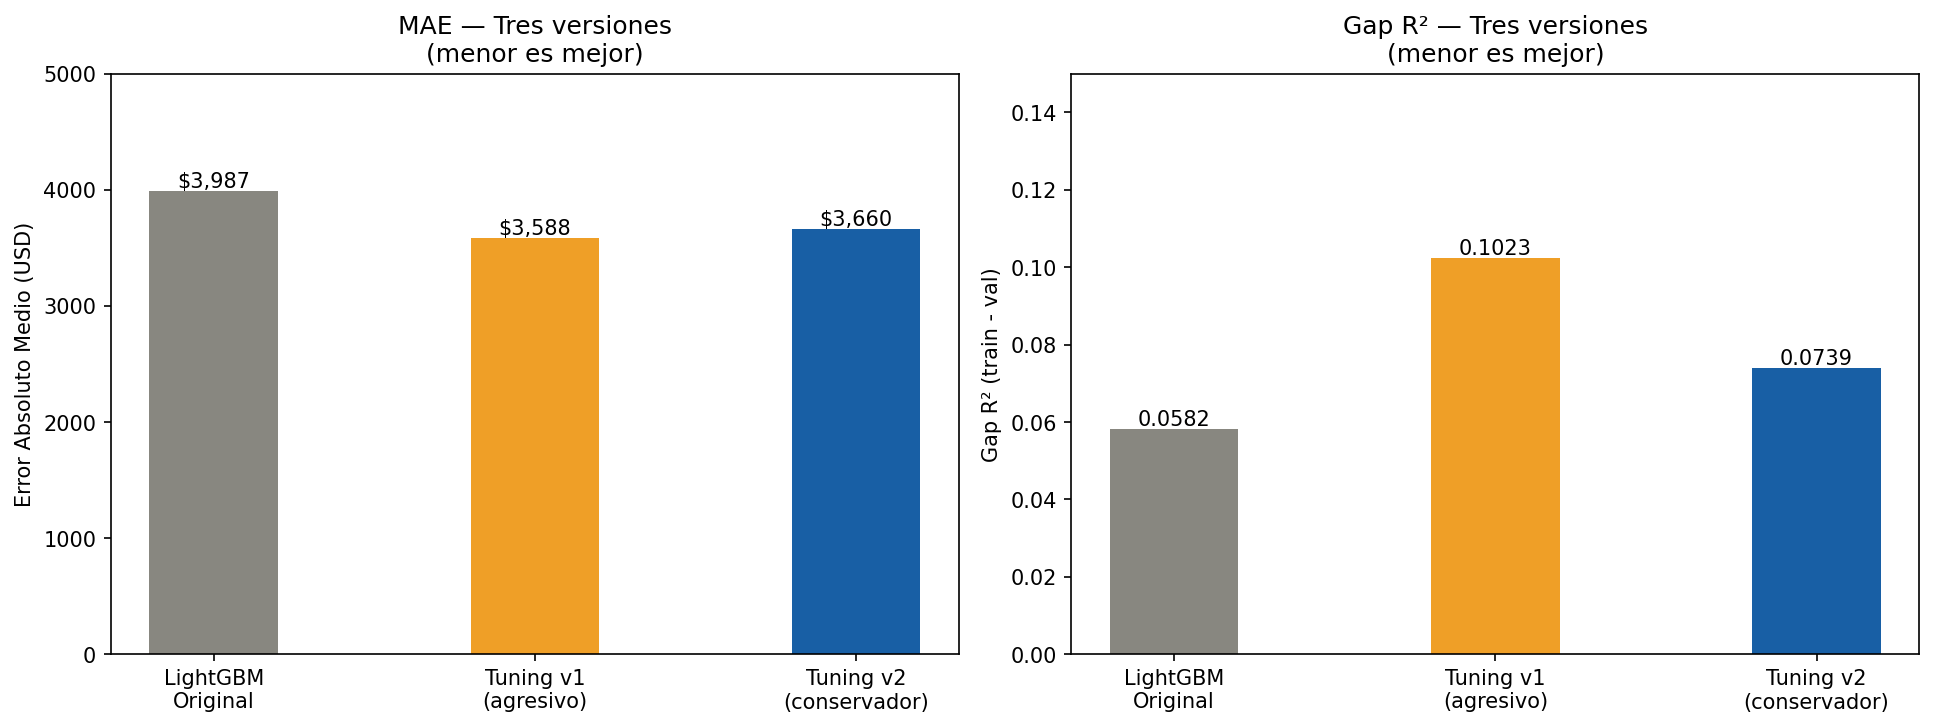
\includegraphics[width=\columnwidth]{../SegundaEtapa/hypertuning_v2_comparacion.png}
    \caption{MAE y Gap R² para las tres versiones de LightGBM.
    Tuning v2 logra el mejor balance entre precisión y generalización.}
    \label{fig:hypertuning}
\end{figure}


%----------------------------------------
\subsection{Evaluación Final en Test Set}
\label{subsec:test}

El modelo \textit{LightGBM Tuning v2} fue evaluado sobre el conjunto de prueba de 54{,}683 registros (período 2021-05-03 al 2021-05-05), que permaneció bloqueado durante todo el desarrollo anterior. Los resultados se presentan en la Tabla~\ref{tab:test}.

\begin{table}[H]
    \centering
    \caption{Métricas del modelo final en Test Set vs Validation Set}
    \label{tab:test}
    \begin{tabular}{lrrr}
        \toprule
        \textbf{Métrica} & \textbf{Val} & \textbf{Test} & \textbf{Diferencia} \\
        \midrule
        MAE  (\$) & 3{,}660 & 3{,}999 & +339 (+9.3\%) \\
        RMSE (\$) & 6{,}309 & 6{,}917 & +608 (+9.6\%) \\
        R²        & 0.792   & 0.762   & $-$0.030      \\
        \bottomrule
    \end{tabular}
\end{table}

El MAE en test (\$3{,}999) representa una mejora del 27.4\% respecto al mejor baseline (Regresión Lineal, \$5{,}510). La diferencia entre validación y test es de \$339 en MAE (9.3\%), lo que confirma que el modelo generaliza adecuadamente a datos no vistos bajo el esquema de partición temporal adoptado. La caída de R² de 0.792 a 0.762 es consistente con el desplazamiento temporal entre los conjuntos, los anuncios de mayo de 2021 presentan una distribución de precios levemente diferente a la de abril, efecto esperable en datos de mercado con variación temporal.

La distribución de errores muestra una media de \$24, lo que indica que el modelo no presenta sesgo sistemático de sobreestimación ni subestimación. La curva de errores acumulados revela que el 80\% de las predicciones tienen un error absoluto menor a \$6{,}000.

\begin{figure}[H]
    \centering
    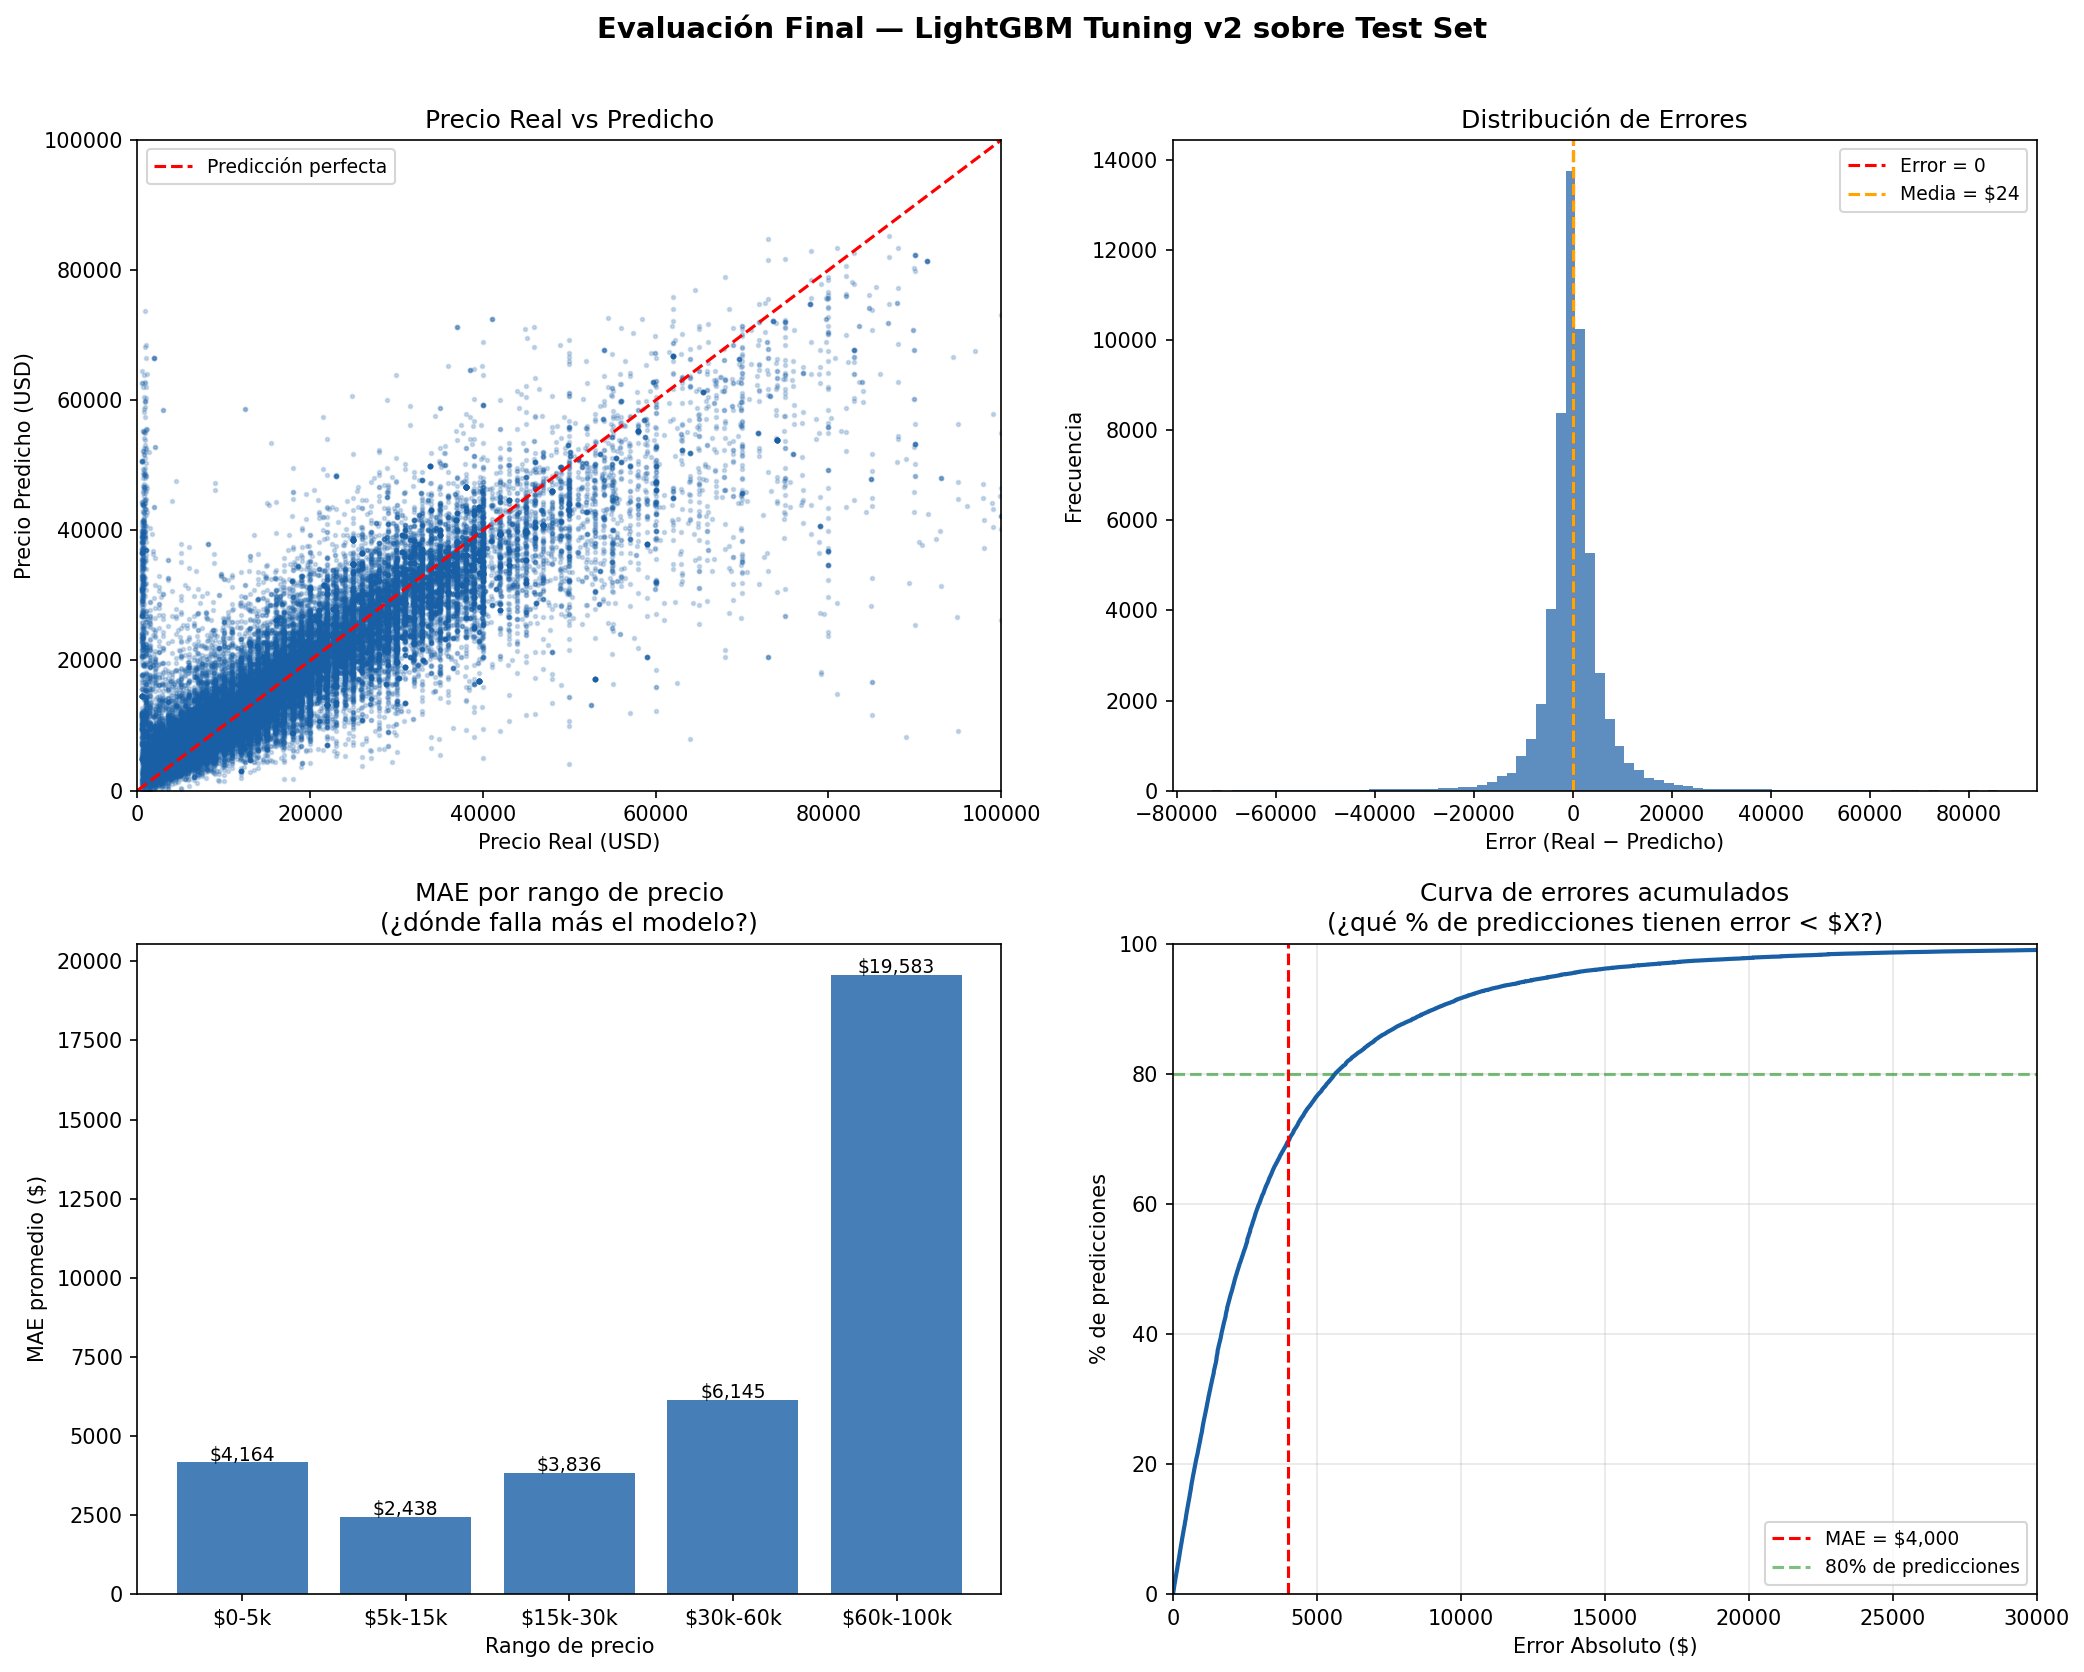
\includegraphics[width=\columnwidth]{../SegundaEtapa/evaluacion_final_test.png}
    \caption{Evaluación final del modelo sobre el test set. (a) Precio real vs predicho. (b) Distribución de errores centrada en \$24. (c) MAE por rango de precio. (d) Curva de errores acumulados.}
    \label{fig:eval_final}
\end{figure}


%----------------------------------------------------
\subsection{Análisis por Rango de Precio}
\label{subsec:rangos}

La Tabla~\ref{tab:rangos} desagrega el MAE por segmento de precio para identificar dónde el modelo presenta mayor y menor precisión.

\begin{table}[H]
    \centering
    \caption{MAE y error porcentual por rango de precio en Test Set}
    \label{tab:rangos}
    \begin{tabular}{lrrr}
        \toprule
        \textbf{Rango} & \textbf{Registros} & \textbf{MAE (\$)} & \textbf{Error (\%)} \\
        \midrule
        \$0 – \$5k    & 9{,}579  & 4{,}164  & 370.5 \\
        \$5k – \$15k  & 19{,}307 & 2{,}438  & 26.4  \\
        \$15k – \$30k & 16{,}150 & 3{,}836  & 17.7  \\
        \$30k – \$60k & 8{,}863  & 6{,}145  & 15.3  \\
        \$60k – \$100k& 784      & 19{,}583 & 26.0  \\
        \bottomrule
    \end{tabular}
\end{table}

El segmento \$5{,}000–\$15{,}000 presenta el mejor rendimiento con un MAE de \$2{,}438 y un error porcentual del 26.4\%. Este rango concentra el 35.3\% de los registros del test set, lo que lo convierte en el segmento más relevante para el sistema de recomendación dado que corresponde al mercado de mayor volumen de transacciones en Craigslist. El rendimiento degradado en el segmento \$60{,}000–\$100{,}000 (MAE de \$19{,}583) se atribuye a la baja representación de ese rango en el dataset: solo 784 registros en el test set (1.4\%) frente a 19{,}307 en el segmento de mayor volumen.

El error porcentual del 370.5\% en el segmento \$0–\$5{,}000 no refleja una limitación del modelo sino una limitación del dataset: anuncios con precios simbólicos (\$838, \$883, \$1{,}008) pero con características de vehículos de alto valor que sobrevivieron los filtros de limpieza. Estos casos se analizan en detalle en la Sección~\ref{sec:discusion}.

%----------------------------------------------------
\subsection{Análisis de Explicabilidad SHAP}
\label{subsec:res_shap}

El análisis SHAP sobre una muestra de 2{,}000 registros del test set revela la importancia global de cada variable y su dirección de influencia sobre el precio predicho. La Tabla~\ref{tab:shap} presenta el ranking de las diez variables más influyentes medido como el promedio del valor absoluto de SHAP.

\begin{table}[H]
    \centering
    \caption{Top 10 variables por importancia SHAP promedio}
    \label{tab:shap}
    \begin{tabular}{lr}
        \toprule
        \textbf{Variable} & \textbf{Importancia SHAP (\$)} \\
        \midrule
        year              & 6{,}054 \\
        odometer          & 3{,}188 \\
        cylinders         & 2{,}560 \\
        fuel\_gas         & 2{,}070 \\
        drive\_fwd        & 1{,}565 \\
        type\_sedan       & 526     \\
        fuel\_other       & 518     \\
        type\_pickup      & 325     \\
        transmission\_other & 303   \\
        type\_truck       & 303     \\
        \bottomrule
    \end{tabular}
\end{table}

Las variables \texttt{year} y \texttt{odometer} dominan el ranking con importancias de \$6{,}054 y \$3{,}188 respectivamente, confirmando las correlaciones identificadas en el EDA de la Etapa 1 ($r{=}0.58$ y $r{=}{-}0.54$). Existe una brecha pronunciada entre las primeras cinco variables (\$1{,}565–\$6{,}054) y el resto (menos de \$530), lo que indica que el precio de un vehículo usado en este dataset está determinado principalmente por cinco factores: año de fabricación, kilometraje, número de cilindros, tipo de combustible y tracción.

\begin{figure}[H]
    \centering
    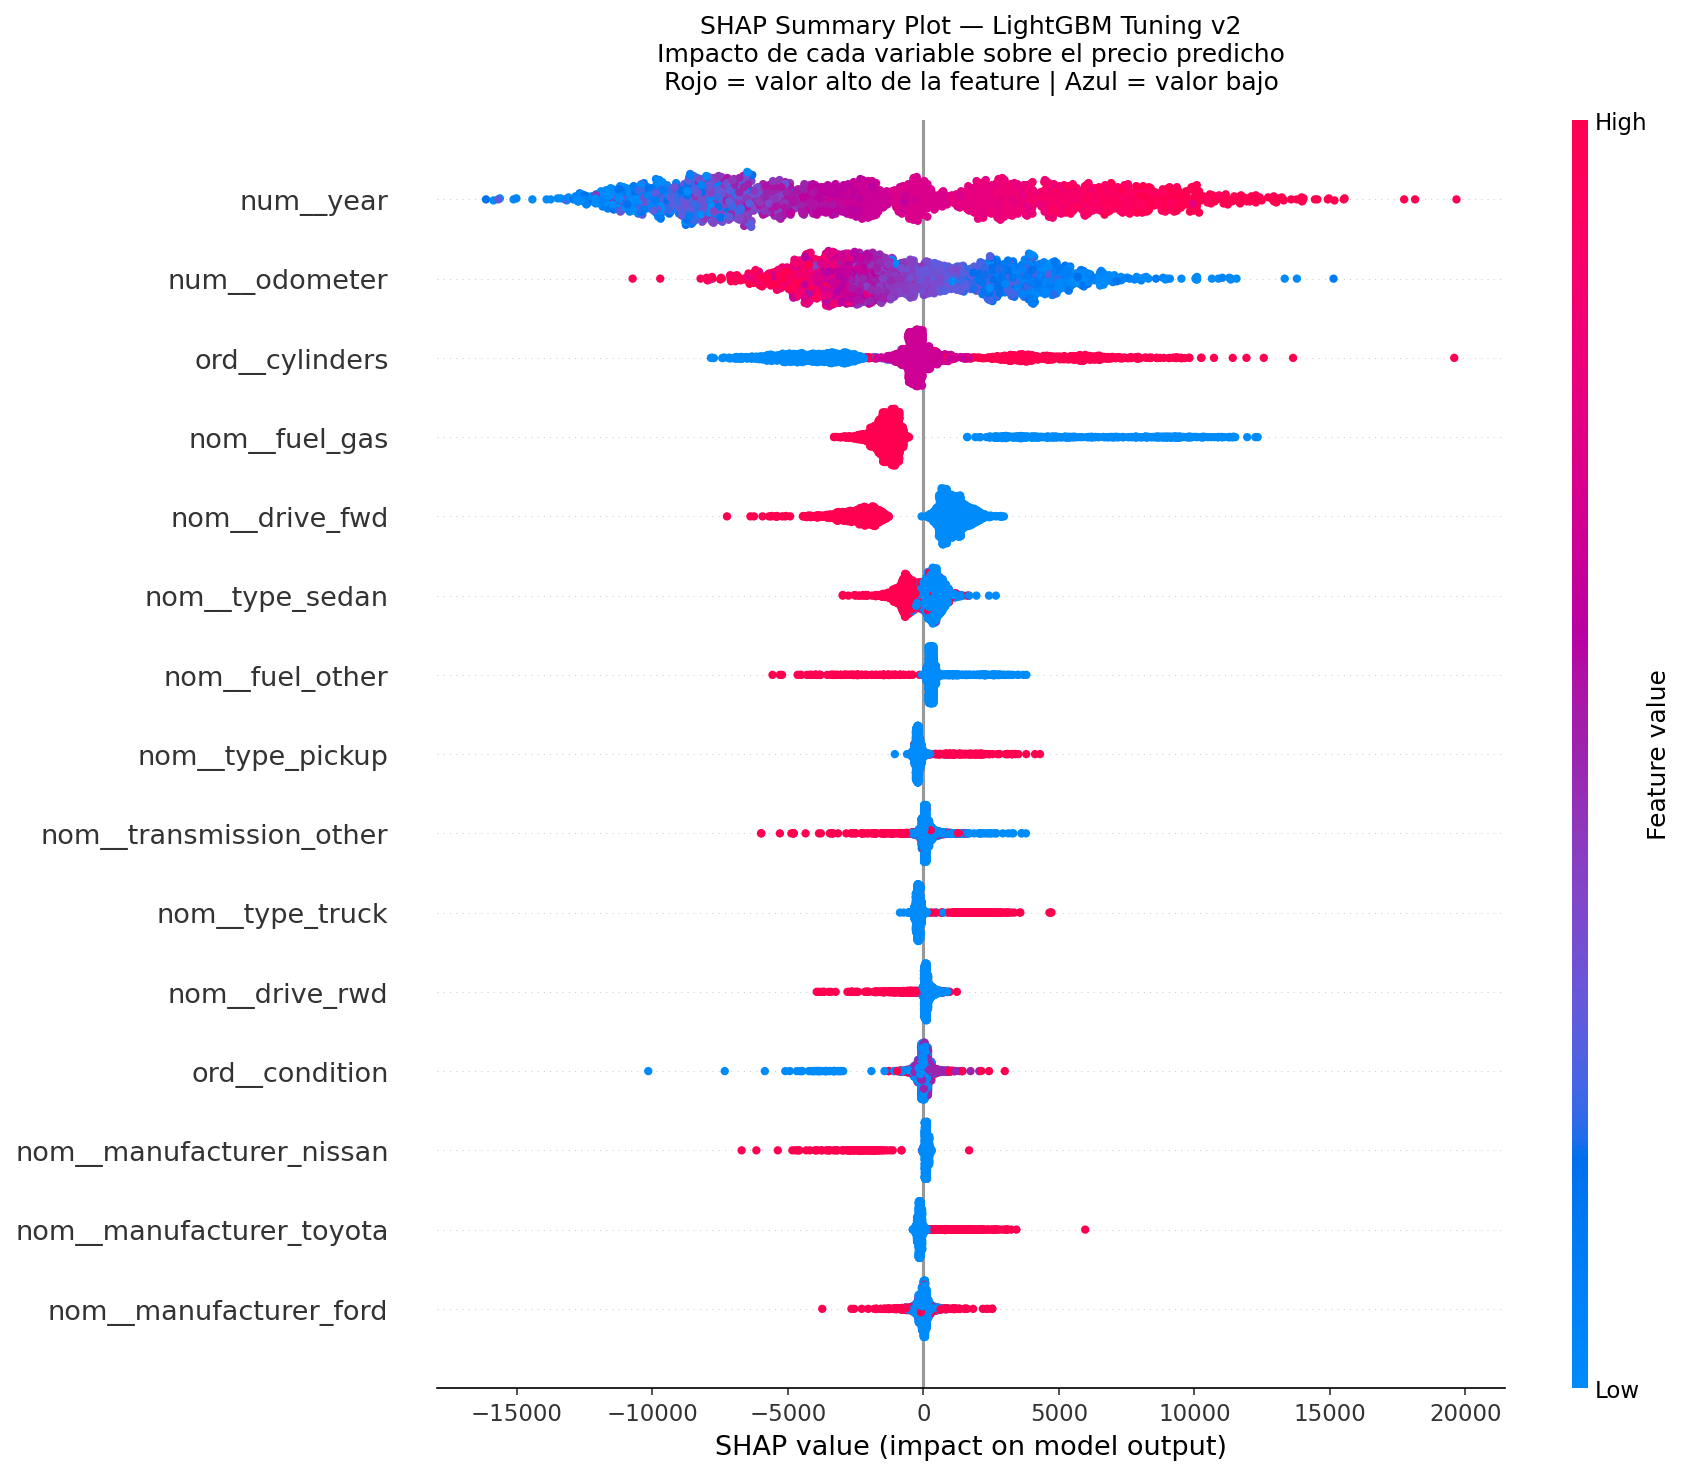
\includegraphics[width=\columnwidth]{../SegundaEtapa/shap_summary_plot.png}
    \caption{SHAP Summary Plot sobre 2{,}000 registros del test set. Rojo = valor alto de la feature, Azul = valor bajo. El eje horizontal representa el impacto en dólares sobre el precio predicho.}
    \label{fig:shap_summary}
\end{figure}

El \textit{waterfall plot} (Fig.~\ref{fig:shap_waterfall}) ilustra la predicción del vehículo con precio más cercano a la mediana del mercado. El modelo parte de un precio base de \$19{,}809 (promedio del dataset) y ajusta hacia abajo por ser marca Chrysler ($-$\$3{,}287), tracción delantera ($-$\$2{,}004) y combustible gasolina ($-$\$1{,}317), mientras que el bajo kilometraje (+\$797) y el tipo de vehículo (+ \$758) contribuyen positivamente. El precio predicho resultante es \$14{,}287 frente a un precio real de \$14{,}444, con un error de \$157.

\begin{figure}[H]
    \centering
    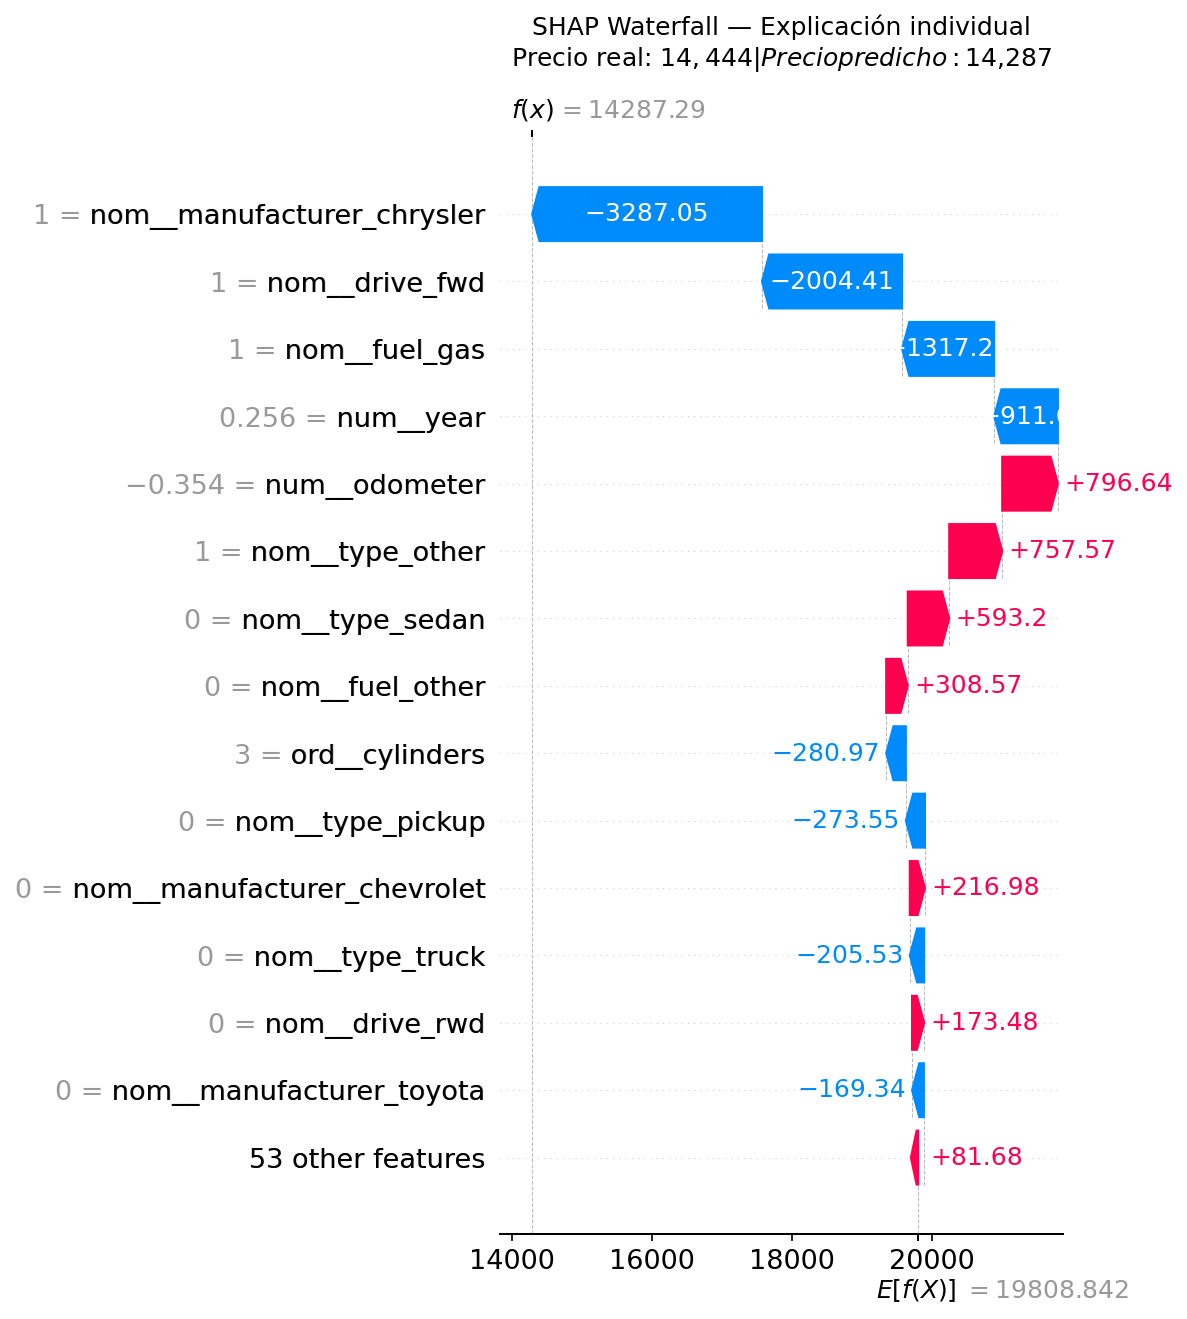
\includegraphics[width=\columnwidth]{../SegundaEtapa/shap_waterfall_v2.png}
    \caption{SHAP Waterfall para el vehículo con precio más cercano a la mediana (\$14{,}444). Precio base: \$19{,}809. Precio predicho: \$14{,}287. Error: \$157.}
    \label{fig:shap_waterfall}
\end{figure}

%----------------------------------------------------
\subsection{Resultados del Agente Inteligente}
La validación del agente se realizó mediante dos sesiones de prueba estructuradas con un total de 21 turnos de conversación: una sesión exploratoria de 6 turnos y una sesión extendida de 15 turnos. Cada turno fue registrado automáticamente en formato JSON por el módulo \texttt{RegistradorEjecucion}, capturando la consulta del usuario, la tarea inferida por el \textit{Planner}, los parámetros extraídos, el resultado del \textit{Executor}, el veredicto del \textit{Verifier} y el tiempo de respuesta de extremo a extremo.

\subsubsection{Escenarios de Prueba}
Los 21 turnos cubrieron las tres tareas disponibles del agente con escenarios representativos del uso real del sistema. Para \texttt{buscar\_vehiculos} se evaluaron consultas con múltiples restricciones simultáneas (tipo, transmisión, presupuesto, fabricante), una consulta imposible de satisfacer (Ferrari eléctrico por menos de \$5{,}000) para verificar el comportamiento ante disponibilidad nula, y consultas con parámetros no soportados por la herramienta como \texttt{drive} y \texttt{odometer}, que revelaron una limitación en el mapeo entre el \textit{Planner} y el \textit{Executor}. Para \texttt{estimar\_precio} se probaron vehículos de distintos segmentos de precio: un Toyota Camry 2019 (\$26{,}461), un Ford F-150 2019 en condición excelente (\$42{,}185), un Honda Civic 2018 con conversión de kilómetros a millas (\$18{,}863) y un Tesla Model 3 2021 eléctrico (\$41{,}644). Para \texttt{explicar\_prediccion} se validó tanto la recuperación de contexto conversacional; el agente respondió correctamente a preguntas como ``¿por qué ese carro vale eso?'' sin que el usuario repitiera las características del vehículo; como la coherencia de los valores SHAP retornados, que en todos los casos identificaron \texttt{year} como el factor de mayor contribución al precio.

\subsubsection{Métricas de Validación}
La Tabla~\ref{tab:metricas_agente} resume las métricas de validación agregadas por tarea sobre las dos sesiones combinadas.

\begin{table}[h]
    \centering
    \caption{Métricas de validación del agente por tarea }
    \label{tab:metricas_agente}
    \begin{tabular}{lcccc}
        \hline
        \textbf{Tarea} & \textbf{Turnos} & \textbf{Éxito(\%)} &
        \textbf{Reintentos} & \textbf{Tiempo avg.(s)} \\
        \hline
        {buscar\_vehiculos}    & 8 & 62.5  & 0.75 & 328.9 \\
        {estimar\_precio}      & 7 & 100.0 & 0.00 & 585.8 \\
        {explicar\_prediccion} & 6 & 100.0 & 0.00 & 275.4 \\
        \hline
        \textbf{Total}                & 21 & 81.0 & 0.29 & 393.7 \\
        \hline
    \end{tabular}
\end{table}

Las tareas \texttt{estimar\_precio} y \texttt{explicar\_prediccion} alcanzaron una tasa de éxito del 100\%, como se observa en la Figura~\ref{fig:tasa_exito}. Los 3 fallos registrados correspondieron exclusivamente a \texttt{buscar\_vehiculos} y se originaron en dos causas distintas: un turno con disponibilidad nula en el dataset (Ferrari eléctrico por menos de \$5{,}000, cuyo inventario es inexistente en el mercado de Craigslist de 2021), y dos turnos donde el \textit{Planner} extrajo parámetros válidos semánticamente (\texttt{drive}, \texttt{odometer}) pero no soportados por la firma de la función \texttt{buscar\_vehiculos}, provocando excepciones en el \textit{Executor} que el mecanismo de reintento del \textit{Verifier} no pudo resolver al no modificar los parámetros incompatibles.

Respecto al tiempo de respuesta, la Figura~\ref{fig:tiempos} muestra que la distribución presenta asimetría positiva: la mayoría de lo turnos (11 de 21) se completaron en menos de 300 segundos, mientras que cuatro turnos superaron los 600 segundos. La latencia elevada se atribuye al procesamiento local del modelo Qwen3 mediante Ollama sin aceleración por GPU, y no a la inferencia del modelo LightGBM ni a las búsquedas en el dataset, que se ejecutan en milisegundos. 

\begin{figure}[h]
    \centering
    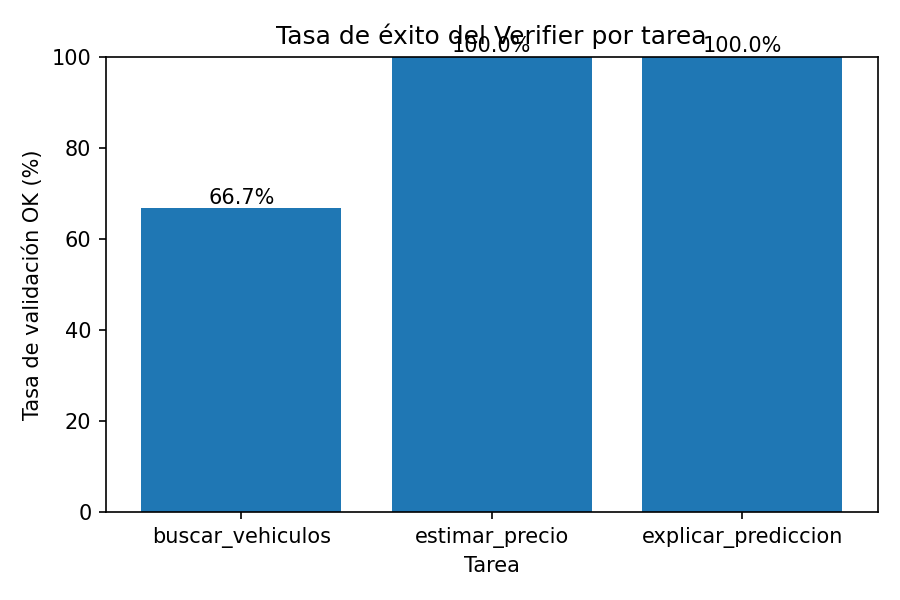
\includegraphics[width=0.48\textwidth]{../agente/logs/figuras/exito_por_tarea.png}
    \caption{Tasa de éxito del Verifier por tarea sobre 21 turnos de prueba.}
    \label{fig:tasa_exito}
\end{figure}

\begin{figure}[h]
    \centering
    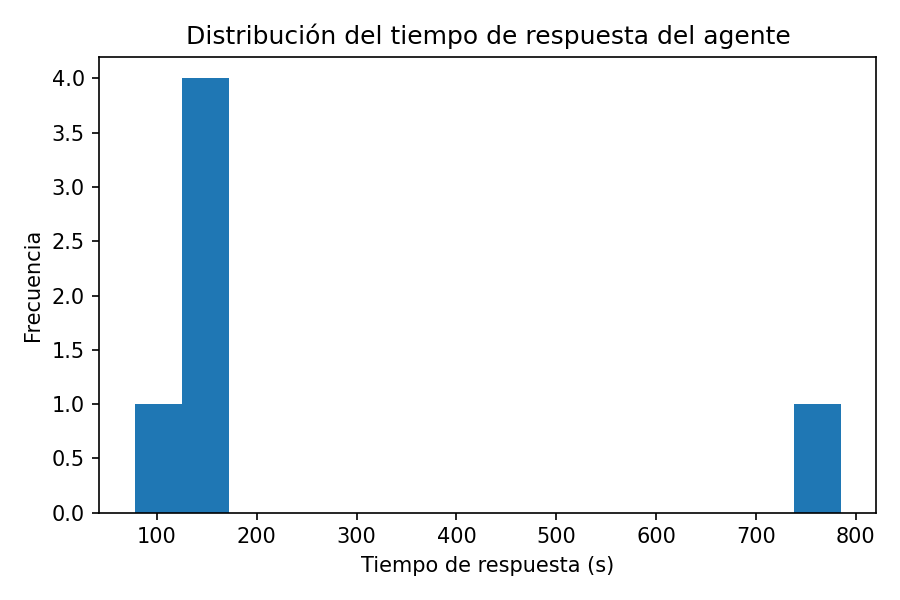
\includegraphics[width=0.48\textwidth]{../agente/logs/figuras/distribucion_tiempos.png}
    \caption{Distribución del tiempo de respuesta del agente por turno.
    La mayoría de las consultas se resuelven en menos de 300 segundos con el LLM ejecutado localmente sin GPU.}
    \label{fig:tiempos}
\end{figure}


% DISCUSIÓN
\section{Discusión}
\label{sec:discusion}

%----------------------------------------------------
\subsection{Hallazgos de Explicabilidad (SHAP)}
\label{subsec:disc_shap}

El análisis SHAP sobre el modelo final \textit{LightGBM Tuning v2} permite validar que el modelo aprendió relaciones económicamente coherentes con el mercado de vehículos usados, y revela hallazgos que no eran evidentes en el análisis exploratorio inicial.

\textbf{Hallazgo 1: Dominio de variables mecánicas básicas.} 

El año de fabricación (\texttt{year}) y el kilometraje (\texttt{odometer}) lideran el ranking con importancias SHAP de \$6{,}054 y \$3{,}188 respectivamente, confirmando las correlaciones identificadas en el EDA ($r{=}0.58$ y $r{=}{-}0.54$). El \textit{summary plot} (Fig.~\ref{fig:shap_summary}) muestra que vehículos con año de fabricación reciente; representados en rojo; acumulan valores SHAP positivos de hasta \$20{,}000, mientras que vehículos con años antiguos; representados en azul; presentan valores negativos de hasta $-$\$15{,}000. El odómetro exhibe el patrón inverso, mayor kilometraje reduce el precio predicho, consistente con la depreciación por uso documentada en el mercado automotriz \cite{aggarwal2016}.

\textbf{Hallazgo 2: Importancia del número de cilindros.} 

La variable \texttt{cylinders} ocupa la tercera posición con una importancia SHAP de \$2{,}560, superando a \texttt{condition} (posición 12) y a cualquier marca específica. Este resultado no era predecible a partir del análisis de correlaciones lineales del EDA, donde la variable no presentaba una correlación directa con el precio comparable a la de \texttt{year} u \texttt{odometer}. SHAP captura la interacción no lineal entre cilindros y otras variables: motores de mayor cilindrada no solo implican un precio más alto de forma directa, sino que se asocian con tipos de vehículo (pickup, SUV, camión) que retienen mejor su valor en el mercado estadounidense.

\textbf{Hallazgo 3: Comportamiento de variables de combustible y tracción.} 

La variable \texttt{fuel\_gas} (combustible gasolina) presenta valores SHAP negativos para la mayoría de los registros, lo que indica que ser de gasolina baja el precio predicho relativo al promedio. Este resultado es contraintuitivo en un primer análisis pero tiene una explicación estructural. Los vehículos de combustible alternativo (diesel, híbrido, eléctrico) tienen precios promedio más altos en el dataset dado que son modelos más recientes o de gama superior. De forma análoga, la tracción delantera (\texttt{drive\_fwd}) contribuye negativamente al precio, en contraste con la tracción integral (4WD) y trasera (RWD) que se asocian a vehículos de mayor valor.

\textbf{Hallazgo 4: Ausencia de patrones espurios.}

El ranking de importancia SHAP no presenta variables con alta influencia que carezcan de justificación económica. Si el modelo hubiera aprendido patrones falsos derivados de data leakage o de correlaciones falsas en el dataset, variables como \texttt{region}, \texttt{state} o \texttt{posting\_date}; excluidas explícitamente del pipeline; habrían aparecido en posiciones superiores. La coherencia del ranking con el conocimiento del dominio valida que el protocolo de prevención de data leakage descrito en la Subsección~\ref{subsec:particion} fue efectivo.

\textbf{Análisis individual: waterfall plot.}

El \textit{waterfall plot} (Fig.~\ref{fig:shap_waterfall}) ilustra la descomposición de la predicción para el vehículo con precio más cercano a la mediana del mercado (\$14{,}444). Partiendo del precio base de \$19{,}809, las características del vehículo ajustan la predicción hacia abajo en \$5{,}522 netos, eso quiere decir que la marca Chrysler resta \$3{,}287, la tracción delantera resta \$2{,}004 y el combustible gasolina resta \$1{,}317, mientras que el bajo kilometraje aporta +\$797 y el tipo de carrocería aporta +\$758. El precio predicho resultante (\$14{,}287) difiere del precio real en solo \$157, con todos los ajustes siendo económicamente justificables.

%----------------------------------------------------
\subsection{Limitaciones}
Existen límites dentro del modelo asociados a los sesgos. Primero, existe una representación limitada de ciertas categorías.  Los vehículos que están bajo la categoría de new en cuanto a la condición (0.26\% del dataset) tienen un MAE de alrededor de \$9 000, mientras que el  MAE global es de \$4 000. Esto lo que quiere dar a entender es que el modelo  discrimina a los casos en los que un usuario quiere vender un vehículo nuevo o buscar vehículos nuevos. Por otro lado, los vehículos eléctricos solamente representan el 0.42\% del dataset por lo que las recomendaciones del agente para este conjunto de vehículo es menos confiable. Este es un segmento importante ya que en los  últimos años ha tenido un fuerte crecimiento en el mercado. También se presenta una limitación geográfica ya que el dataset proviene exclusivamente de Craigslist en Estados Unidos. Por lo tanto, el modelo no es transferible a otros mercados sin reentrenamiento. Asimismo, se presenta una cobertura desigual entre fabricantes debido a que Ford y Chevrolet dominan con más del 30\% de los registros combinados. El modelo tiene mayor precisión para estas marcas que para fabricantes con pocos registros como Ferrari o Maserati, lo que podría perjudicar a usuarios interesados en vehículos específicos que no aparecen tanto en el dataset. Finalmente, hay que tomar en consideración que el dataset contiene información correspondiente al año 2021. Los precios del mercado de vehículos usados han cambiado significativamente desde entonces. El usuario debe saber que las estimaciones reflejan el mercado de 2021 y no el mercado actual para evitar confusiones

\subsection{Trade-off del Hypertuning: MAE vs Gap R²}
\label{subsec:disc_hypertuning}
El proceso de optimización de hiperparámetros ilustra un trade-off  fundamental en el aprendizaje automático: la tensión entre minimizar el error en los datos disponibles y maximizar la capacidad de generalización a datos futuros. La primera ronda de búsqueda (\textit{Tuning v1}) encontró parámetros que optimizan agresivamente el MAE reducción de \$399 respecto al modelo base pero a costa de un incremento del Gap R² de 0.058 a 0.102. Esta configuración, caracterizada por un \texttt{learning\_rate} de 0.181 y \texttt{num\_leaves} de 118, genera árboles complejos que aprenden patrones muy específicos del conjunto de entrenamiento que no se replican en datos nuevos.

La segunda ronda (\textit{Tuning v2}), con rangos de búsqueda más conservadores, encontró un punto de equilibrio: un MAE de \$3{,}660 (mejora de \$327 respecto al modelo base) con un Gap R² de 0.074, representando una reducción del 27.6\% en overfitting respecto a \textit{Tuning v1} a costa de solo \$72 adicionales en MAE. Esta diferencia es menor que la incertidumbre inherente del modelo (MAE $\approx$ \$4{,}000 en test), por lo que la ganancia en generalización justifica ampliamente el sacrificio en precisión teórica. Esto refuerza la importancia del Gap R² como criterio de selección en contextos con datos temporales, donde la distribución del conjunto de prueba puede diferir de la del entrenamiento, como se confirmó con la caída de R² de 0.792 (validación) a 0.762 (test).

\subsection{Implicaciones para el Agente Inteligente}
\label{subsec:disc_agente}
La integración del modelo en el agente LangGraph revela implicaciones tanto técnicas como de usabilidad que van más allá del rendimiento predictivo del modelo aislado. Desde el punto de vista técnico, la arquitectura Planner-Executor-Verifier demostró ser adecuada para este dominio: el \textit{Planner} basado en Qwen3 logró extraer correctamente los parámetros de búsqueda y estimación en la mayoría de los turnos, mientras que el \textit{Verifier} cumplió su función de validación detectando casos límite como consultas con disponibilidad nula e intentando reintentos automáticos con parámetros relajados.

Sin embargo, los resultados de validación evidencian una limitación arquitectural relevante, que el mecanismo de reintento del \textit{Verifier} no puede resolver fallos causados por incompatibilidades entre los parámetros que el \textit{Planner} extrae semánticamente válidos (\texttt{drive}, \texttt{odometer}) y los que acepta la firma de \texttt{buscar\_vehiculos}. Esto sugiere que la interfaz entre el \textit{Planner} y el \textit{Executor} requiere un esquema de validación de parámetros anterior a la ejecución, que podría implementarse como un paso intermedio de normalización dentro del nodo adaptador de \texttt{agente.py} \cite{dong2025, rosario2025}.

Desde la perspectiva del usuario, la capacidad de mantener contexto entre turnos mediante \texttt{MemorySaver} demostró su valor en la sesión extendida, ya que preguntas como ``¿por qué ese Toyota Camry tiene ese precio estimado?'' fueron resueltas correctamente sin que el usuario repitiera las características del vehículo. Esta característica es especialmente valiosa en el flujo natural de una consulta de compra, donde el usuario típicamente explora opciones de forma iterativa. La integración de SHAP como mecanismo de justificación de las predicciones permite al agente no solo recomendar vehículos sino explicar los factores que determinan su valor estimado, alineándose con el principio de IA explicable en sistemas de apoyo a decisiones \cite{masterman2024}.

% CONCLUSIONES
% -----------------------------------------------------
\section{Conclusiones}
\label{sec:conclusiones}

Este trabajo presentó un sistema de recomendación de vehículos usados que integra un modelo predictivo de Machine Learning con un agente inteligente basado en LangGraph. El modelo LightGBM Tuning v2, seleccionado tras la evaluación comparativa de seis algoritmos bajo un protocolo de validación temporal estricto, obtuvo un MAE de \$3{,}999 y un R² de 0.762 sobre el conjunto de prueba, representando una mejora del 27.4\% respecto al baseline de regresión lineal. El protocolo de partición temporal y la prevención explícita de \textit{data leakage} garantizaron que estas métricas reflejan el rendimiento real esperado en producción.

El análisis de explicabilidad con SHAP confirmó que el modelo aprendió relaciones económicamente coherentes; el año de fabricación y el kilometraje dominan las predicciones con importancias SHAP de \$6{,}054 y \$3{,}188 respectivamente, en línea con las correlaciones identificadas en el análisis exploratorio ($r{=}0.58$ y $r{=}{-}0.54$). El hallazgo más relevante fue la posición del número de cilindros (importancia SHAP de \$2{,}560) por encima de variables intuitivamente más prominentes como la condición del vehículo, lo que demuestra el valor de SHAP para revelar relaciones no lineales que los análisis de correlación tradicionales no capturan.

La integración en el agente LangGraph con arquitectura Planner-Executor-Verifier validó la viabilidad de consumir el modelo predictivo como herramienta de un sistema conversacional. Sobre 21 turnos de prueba estructurada, el agente alcanzó una tasa de éxito global del 81\%, con 100\% en las tareas de estimación de precio y explicación de predicciones. La memoria persistente entre turnos permitió conversaciones iterativas donde el usuario puede explorar y refinar sus consultas sin repetir información, replicando el flujo natural de una consulta de compra de vehículo.

Como trabajo futuro, se identifican tres líneas de mejora prioritarias. Primero, ampliar la interfaz de \texttt{buscar\_vehiculos} para aceptar parámetros adicionales como tracción y kilometraje máximo, que el \textit{Planner} ya extrae correctamente pero el \textit{Executor} no puede procesar actualmente. Segundo, incorporar datos más recientes al dataset de entrenamiento, dado que los precios del mercado de vehículos usados han cambiado significativamente desde 2021. Tercero, reducir la latencia del agente mediante GPU dedicada o APIs de LLM en la nube, donde el tiempo de respuesta promedio de 393.7 segundos podría reducirse por un factor de 10 o más, haciendo el sistema viable para uso interactivo en tiempo real.

% REFERENCIAS
% -----------------------------------------------------
\begin{thebibliography}{99}

\bibitem{aggarwal2016}
C.~C. Aggarwal,
\textit{Recommender Systems: The Textbook}.
Springer, 2016.

\bibitem{lundberg2017}
S.~M. Lundberg and S.-I. Lee,
``A unified approach to interpreting model predictions,''
in \textit{Advances in Neural Information Processing Systems},
vol.~30, pp.~4765--4774, 2017.

\bibitem{chen2016}
T.~Chen and C.~Guestrin,
``XGBoost: A scalable tree boosting system,''
in \textit{Proc. 22nd ACM SIGKDD}, pp.~785--794, 2016.

\bibitem{ke2017}
G.~Ke, Q.~Meng, T.~Finley, T.~Wang, W.~Chen, W.~Ma, Q.~Ye, and T.-Y.~Liu,
``LightGBM: A highly efficient gradient boosting decision tree,''
in \textit{Advances in Neural Information Processing Systems},
vol.~30, pp.~3146--3154, 2017.

\bibitem{cui2022}
B.~Cui, Z.~Ye, H.~Zhao, Z.~Renqing, L.~Meng, and Y.~Yang,
``Used car price prediction based on the iterative framework of
XGBoost+LightGBM,''
\textit{Electronics}, vol.~11, no.~18, p.~2932, 2022.

\bibitem{sulianta2024}
F.~Sulianta, E.~Amalia, and A.~Arif,
``Analysis of consumer preferences for used cars using k-means clustering,''
\textit{The Indonesian Journal of Computer Science}, 2024.

\bibitem{ijert2022}
``Forecasting vehicle prices using machine learning techniques,''
\textit{International Journal of Engineering Research \& Technology},
vol.~11, 2022.

\bibitem{schick2023}
T.~Schick et al.,
``Toolformer: Language models can teach themselves to use tools,''
in \textit{Advances in Neural Information Processing Systems},
vol.~36, 2024.

\bibitem{dong2025}
S.~Dong, M.~Zhang, P.~He, B.~Thuraisingham, H.~Liu, and Y.~Xing,
``PEAR: Planner-Executor Agent Robustness Benchmark,''
pp.~4547--4567, 2025.
\url{https://doi.org/10.48550/arxiv.2510.07505}

\bibitem{rosario2025}
R.~F. D.~Rosario, K.~Krawiecka, and C.~S. De~Witt,
``Architecting Resilient LLM Agents: A Guide to Secure 
Plan-then-Execute Implementations,''
\textit{ArXiv}, abs/2509.08646, 2025.
\url{https://doi.org/10.48550/arxiv.2509.08646}

\bibitem{masterman2024}
T.~Masterman, S.~Besen, M.~Sawtell, and A.~Chao,
``The Landscape of Emerging AI Agent Architectures for Reasoning, 
Planning, and Tool Calling: A Survey,''
\textit{ArXiv}, abs/2404.11584, 2024.
\url{https://doi.org/10.48550/arxiv.2404.11584}

\bibitem{chu2024}
W.~Chu, S.~Yin, L.~Huang, L.~Lin, X.~Wang, Z.~Zhang, and H.~Li,
``Verify-Agent: Large Language Model Multi-Agent for Intelligent 
Verification,''
in \textit{2024 International Conference on Ubiquitous Computing 
and Communications (IUCC)}, pp.~374--379, 2024.
\url{https://doi.org/10.1109/iucc65928.2024.00072}

\end{thebibliography}

\end{document}